\documentclass[12pt,a4paper,titlepage]{article}
\usepackage[spanish]{babel} %Seteo el idioma
\usepackage[utf8]{inputenc} %Es para escribir con acentos
\usepackage{titling}
\usepackage{graphicx} %Es para insertar gráficos
\usepackage{siunitx}  %Es para usar notación cintífica
\usepackage{float} %Es para usar el módulo float
\usepackage{slashbox} %Es para tirar mágia en las tablas
\usepackage{multirow}

\begin{document}
%Defino el título y autores
\title{%
	Tópicos de Programación para Científicos Computacionales\\
	\large Informe del Trabajo Práctico Final}
	
\author {Eduador Agustín Rosselot$^{1-3}$ y Maximiliano Jose Perez Frasette$^{2-3}$\\ 
	\small{$^{1}$earosselot@gmail.com [924/11]}\\
	\small{$^{2}$maxi.perezfrasette@gmail.com [862/12]}\\
	\small{$^{3}$Grupo 1 - Alumnos de doctorado del Departamento de Geología}\\
	}
\date{Diciembre 2019}

\maketitle


\section{Ejercicio 1: Dividir y Conquistar}

El archivo donde se encuentran las implementaciones del ejercicio 1 está incluído en el repositorio con el nombre \textit{Ejercicio1.py}, dentro de la carpeta \textbf{src\_ej1}. En esa misma carpeta, se encuentra el gráfico generado (bajo el nombre de \textit{GraficoEj1.png})y un archivo llamado \textit{datosGrafico1.txt} , con los tiempos de cómputo obtenidos. También está incluído el archivo \textit{datitos.txt}, que son los datos suministrados junto con el tp.\par

El código donde están las funciones implementadas se encuentra divido en cuatro secciones. En la primer sección se encuentran las funciones principales, en la segunda sección están todas las funciones auxiliares necesarias para implementar las funciones principales. En la tercer sección se encuentran las funciones implementadas para analizar los diferentes tiempos de ejecución. Por último, en la cuarta sección están los comandos para obtener el gráfico. Cada sección está dividida por un comentario que las identifica claramente. \par

En la sección número uno están las tres funciones principales pedidas por el enunciado del tp, \texttt{listadepuntos(fn)}, \texttt{distanciaMinima(l)} y \texttt{distancia MinimaDyC(l,algoritmo)}. La implementación de las primeras dos funciones es relativamente sencilla. \texttt{Listadepuntos(fn)} utiliza la función auxiliar \texttt{entero(a)}, que convierte \textit{strings} en \textit{floats}. \texttt{DistanciaMinima(l)} recibe una lista de tuplas e itera la cantidad de veces necesaria para calcular la distancia euclídea entre todos los puntos de la lista.Al finalizar, devuelve el par de puntos más cercanos. Está función necesita como parámetro una lista de al menos dos elementos, en ese caso devuelve ese par de puntos.Además, utiliza la función auxiliar \texttt{distancia(p1,p2)}, la cual calcula la distancia euclídea entre dos pares de coordenadas. Por último, \texttt{distanciaMinimaDyC(l, algoritmo)} también busca el par de puntos más cercano dentro de una lista de puntos l, pero utiliza la técnica de Dividir y Conquistar. Esta función está dividida en dos bloques. En el primer bloque, ordena a la lista de entrada "l" según la coordenada en x. Puede utilizar diferentes técnicas de ordenamiento, las cuales se pasan como argumento. Las técnicas disponibles son: \textit{up-sort},\textit{merge-sort} o el algoritmo por default de python. Para las dos primeras técnicas de ordenamiento, se implementaron cuatro funciones auxiliares (las funciones  \texttt{maxPos(a,b,c)} y \texttt{upSort(l)} para ordenar la lista según la técnica de \textit{up-sort} y  \texttt{merge(l1,l2)} y \texttt{mergeSort(l)} para ordenar la lista según la técnica de \textit{merge-sort}). En el segundo bloque, se hace el llamado de la función auxiliar \texttt{minimaDistRec(l)}, que calcula el par de puntos más cercanos de manera recursiva y según la técnica de divivir y conquistar. El parámetro de entrada l, debe ser una lista ordenada según la coordenada en x. El ordenamiento se lleva a cabo dentro de \texttt{minimaDistanciaDyC(l,algoritmo)} para evitar ordenar una lista que ya está ordenada durante los pasos recursivos. Además, \texttt{minimaDistRec(l)} utiliza la función auxiliar \texttt{paresCruzados(l1,l2,x,dist)}. Esta función auxiliar recibe dos pares de listas ordenadas en la coordenada x, que corresponden con los conjuntos de puntos de izquierda y derecha partidos en el paso de dividir.El punto x, mediante el cual se hizo la división y la minima distancia entre los pares de puntos de ambas listas. Está función implemente el paso de combinar, y devuelve posibles pares de coordenadas que podrían encontrarse a una distancia menor a la hallada hasta ese momento (mezcla pares de puntos de los grupos izquierda y derecha)\par 
En la tercera sección del código, se encuentran implementadas las funciones \texttt{puntosAleatorios(a,b)} y \texttt{experimentarAlgoritmos()}. La primer función genera un set de puntos de cantidad a. Los posibles valores de las coordenadas varían  entre -b y b. La segunda función testea a los algoritmo para diferentes sets de datos y devuelve un archivo .txt con los tiempos de ejecución de cada algoritmo. \par 

A continuación se presentan los gráficos de tiempos obtenidos para diferentes cantidades de datos y para diferentes algoritmos empleados. Se tomó como criterio analizar a partir de 1000 puntos, porque para cantidades menores la medición del tiempo está dentro del rango de error del módulo time de python. Las mediciones se emplearon varíando los sets de datos en orden creciente (se probó para 1000, 5000, 10000, 15000, 20000 y 50000 puntos, ver Figura 1). \par 

\begin{figure}[h]
  \centering
    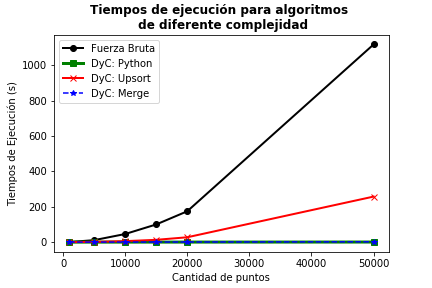
\includegraphics[width=0.8\textwidth]{GraficosEj1}
  \caption{Tiempos de ejecución obtenidos para los diferentes algoritmos}
  \label{fig:ejemplo}
\end{figure}


Como se observa en la Figura 1, a medida que crece el número de datos a calcular, aumenta el tiempo de cómputo para todas las funciones. La función más lenta es distanciaMinima(l), la cual utiliza fuerza bruta como algoritmo. Además, como estaba previsto, puede verse que los tiempos de ejecución aumentan cuadráticamente (fuerza bruta es un algoritmo de O($n^{2}$)). Por otro lado, puede observarse que en los algoritmos que resuelven el problema mediante la técnica de dividir y conquistar, los tiempos de computo disminuyen considerablemente (esta técnica tieme complejidad de O(n.log$^{2}$(n)). En particular, si el ordenamiento se lleva a cabo de acuerdo a la técnica de \textit{merge-sort} o mediante el algoritmo por \textit{default} de python, los tiempos de cómputo son más rápido que al utilizar el ordenamiento por \textit{up-sort}.Por un tema de escala, parece que las curvas de \textit{merge-sort} y del algoritmo de python son contaste en tiempo de cómputo, pero ambas sufren un pequeño incremento en tiempo (ver Tabla 1).

\begin{table}[h]
	\begin{center}
		\begin{tabular}{| c | c | c | c | c | c | c | }
			\hline
\textbf{Algoritmo} & \multicolumn{6}{ |c| }{ \textbf{Tiempos de Ejecución (s)}} \\ \hline
Fuerza Bruta & \num{4.5e-01} & \num{1.1e01} & \num{4.1e01} & \num{1e02} & \num{1.8e02} & \num{2.2e03} \\ \hline
DyC:Python & \num{0e01} & \num{4.7e-02} & \num{1.1e-01} & \num{1.6e-01} & \num{2.0e-01} & \num{4.7e-01} \\ \hline
DyC:Up-Sort & \num{6.2e-02} & \num{1.4e01} & \num{5.5e01} & \num{1.3e01} &\num{2.4e01} & \num{2.0e02} \\  \hline
DyC:Merge-Sort& \num{1.6e-02} & \num{7.8e-02} & \num{1.7e-01} & \num{2.7e-01} & \num{3.6e-01} & \num{1.2e-00} \\ \hline
		
		\end{tabular}
		\caption{Tiempos de ejecución para diferentes algoritmos}
		\label{tab:coches}
	\end{center}
\end{table} 


\section{Ejercicio 2: Python y Numba}
Dentro de la carpeta \textbf{src\_2} ubicada en el repositorio, se encuentran los archivos correspondientes del ejercicio 2. El archivo \textit{ej2.py} contiene la implementación de las funciones, mientras que el archivo \textit{ej2\_graf.py} contiene la implementación de los gráficos obtenidos. \par 
El código \textit{ej2.py} esta implementado para correrse por consola.
contiene a las funciones \texttt{gray\_filer(img)} y \texttt{blur\_filter(img)}. Además, se implementó la función \texttt{medirTiempos(fn,*args)}, la cual mide el tiempo de ejecución de los filtros, y la función \texttt{getfilenames(path)}, que devuelve una lista con las rutas de los archivos del tipo requerido, dentro del path. Para correr la función por consola, se necesitan 5 argumentos: la ruta de la imagen junto con su extensión, el número de threads que se quieren correr (solo sirve para escribir el .csv de salida, no cambia la variable de entorno), el número de repeticiones y el nombre del archivo de salida.\par
El archivo de salida es un .csv, separado por ; que sigue la siguiente estructura: tam\_imagen; threads; veces que se repitió el proceso;  media (tiempos gray); desviacion estandar (tiempos gray); minimo (tiempos gray), maximo(tiempos gray); media (tiempos blur); desviacion estandar (tiempos blur); minimo (tiempos blur), maximo(tiempos blur).

Las figuras 2 y 3 contienen los resultados de escalabilidad para los filtros gray y blur. Cada figura contiene ocho gráficos. Cada gráfico representa el tiempo de ejecución del filtro para una determinada resolución de la imagen utilizada en función de la cantidad de núcleos utilizados (las imágenes se encuentra en el repositorio, en la ruta \textit{src\_2/im}). Las pruebas de tiempo se corrieron utilizando la maquinaria de \textit{just in time} y se utilizó  una computadora de 12 núcleos. Observando la figura 2, puede notarse que para imágenes de baja resolución, la paralelización resulta ineficiente, siendo preferible utilizar un sólo núcleo. Por otro lado, para el resto de las resoluciones, la paralelización disminuye los tiempos de ejecución, pero hay una levé tendencia a aumentar el tiempos cuando se utilizan más de 8 núcleos. La figura 3, muestra todos los gráficos homogéneos debido a un tema de escala (hay mucha diferencia entre utilizar un sólo núcleo o paralelizar). En la tabla 2 puede consultarse alguno de los tiempos obtenidos para más detalles.

\begin{table}[H]
	\begin{center}
		\begin{tabular}{| c | c | c | c | c | c |}
			\hline
\backslashbox{\textbf{Resolución}}{\textbf{Núcleos}} & \multicolumn{5}{ |c| }{ \textbf{Tiempos de Ejecución (s)}} \\ \hline
\multirow{2}{0 cm } & 1 & 2 & 4 & 8 & 10 \\ \cline{2-6}
640x480 & 0.1994 & 0.00203 & 0.00208 & 0.00208 & 0.00204 \\ \hline
1280x1024 & 0.6155 & 0.0015 & 0.0161 & 0.00165 & 0.00162 \\  \hline
5120x4096 & 5.2527 & 0.01150 & 0.01042 & 0.01034 & 0.01058 \\ \hline
		
		\end{tabular}
		\caption{Algunos ejemplos de tiempo de ejecución para el filtro blur}
		\label{tab:coches}
	\end{center}
\end{table} 



\begin{figure}[H]
  \centering
    \includegraphics[width=0.9\textwidth]{GráficosGray}
  \caption{Gráficos de escalabilidad para el filtro gray}
  \label{fig:ejemplo}
\end{figure}


\begin{figure}[H]
  \centering
    \includegraphics[width=0.9\textwidth]{GráficosBlur}
  \caption{Gráficos de escalabilidad para el filtro blur}
  \label{fig:ejemplo}
\end{figure}



\section{Ejercicio 3: Backtraking}

Para resolver el ejercicio 3 se implementaron las funciones que se pedian en el enunciado y algunas funciones auxiliares ocultas. Dentro de las funciones auxiliares, un grupo se ocupa del tratamiento booleano de listas (\texttt{\_not\_lista(self, l1), \_and\_listas(self, l1, l2), \_todo\_False(self, l1), \_pos\_true(self, l1)}. Un segundo grupo se ocupa de obtener una lista ordenada en las 4 direcciones de una casilla (i, j) de valores booleanos en funcion de si las casillas adyacentes fueron visitadas o son parte del camino (\texttt{\_getCamino(self, i, j), \_getVisita(self, i, j)}. En tercer lugar se implementó la funcion \texttt{\_mover(self, movimiento, i, j)} que tiene como entradas un numero entre 0 y 3 (movimiento) que indica la direccion en la que debe moverse y una coordenada (i, j), la posicion actual de la rata y genera un cambio de estado del programa (cambio en valores de atributos). Por ultimo, la funcion auxiliar \texttt{\_notescapes(self)} resuelve el problema de que algunos laberintos no tienen paredes en los bordes y esto hacia que la rata tomara posiciones fuera del laberinto. Se implementó de esta manera porque nos pareció mas eficiente cerrar las paredes a poner un condicional mas en cada movimiento. Además, entendemos que las salidas del laberinto no cumplen ninguna función en la manera que está implementado el programa.\par
Con esta implementación el laberinto puede ser resulto en caso de que tenga una solución posible, o no en caso de que no la tenga al correrlo por consola interactiva. Desde la interfaz gráfica, el programa abra y carga el laberinto, pero al tocar el boton de resolver, la rata se mueve un casillero y obtenemos un error de qt que no pudimos solucionar (QObject::startTimer: timers cannot be started from another thread).

\end{document}
